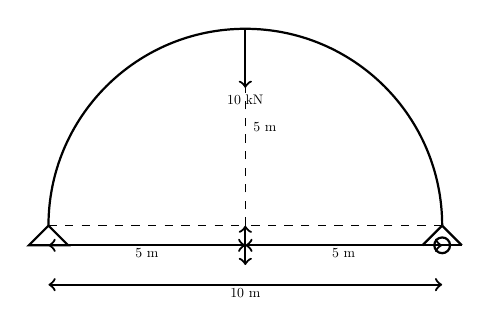
\begin{tikzpicture}[scale=0.5, every node/.style={scale=0.5}]

% Draw the semicircular arch
\draw[thick] (0,0) arc[start angle=180,end angle=0,radius=5];

% Draw supports at the ends of the arch
\draw[thick] (0,0) -- (-0.5,-0.5) -- (0.5,-0.5) -- cycle;  % Left support
\draw[thick] (10,0) -- (9.5,-0.5); % Right support (roller)
\draw[thick] (10,0) -- (10.5,-0.5);
\draw[thick] (9.5,-0.5) -- (10.5,-0.5);
\draw[thick] (10,-0.5) circle (0.2); % Roller circle

% Draw vertical load arrow at the top
\draw[->,thick] (5,5) -- (5,3.5);
\node at (5,3.2) {10 kN};

% Vertical dashed lines from arch to base (distances)
\draw[dashed] (0,0) -- (5,0);
\draw[dashed] (5,0) -- (5,5);
\draw[dashed] (10,0) -- (5,0);

% Draw horizontal dimension lines
\draw[<->,thick] (0,-0.5) -- (5,-0.5);
\node at (2.5,-0.7) {5 m};

\draw[<->,thick] (5,-0.5) -- (10,-0.5);
\node at (7.5,-0.7) {5 m};

\draw[<->,thick] (0,-1.5) -- (10,-1.5);
\node at (5,-1.7) {10 m};

% Draw vertical dimension line
\draw[<->,thick] (5,-1) -- (5,0);
\node at (5.5,2.5) {5 m};

\end{tikzpicture}
